\chapter{Applications, Summary and Conclusions}\label{chap:conclusions}
\begin{epigraphs}
  \qitem{The outcome of any serious research can only be to make two questions grow where only one grew before.}{Thorstein Veblen (1908)}%, The Evolution of the Scientific Point of View, University of California Chronicle.
\end{epigraphs}
% \textit{Chapter in brief: Overall observations and conclusions of the thesis (chapter summaries go in each chapter to make them self contained.) Future work - in CompMusic, rhythm analysis, future directions originating out of thesis, future work that should have been done in the past and might have benefited the work presented in the thesis.}
The concluding chapter of the dissertation aims to present some concrete applications of the rhythm analysis approaches and results presented in the previous chapters. It is followed by a summary of the work presented in the dissertation, along with some key results and conclusions. The thesis opens up a host of open problems - pointers and directions for future work based on the thesis form the last part of the chapter. 
\section{Applications}
There are several applications for the research work presented in the dissertation. Some of these applications have already been identified in \chapref{chap:intro} and \chapref{chap:probdef}. The goal of this section is to present concrete examples of such applications, and further suggest other applications that might be built or get benefited from the work presented here. The section describes some of the applications that have resulted from the work in CompMusic so far, and those that have been planned within the efforts of the project. Possible future applications with the data and methods are also discussed briefly. 

At the outset, the primary objective and application of automatic rhythm analysis is to use it for defining rhythm similarity measures between (and within) music pieces in large collections of music. While this has not been addressed formally in this thesis, there are several ways in which the research discussed in the thesis can be used to define similarity measures and use them for various applications. 
%This section describes some of the applications of the work presented in the dissertation, describing both the applications that have already resulted, and the ones that are planned within the other efforts of CompMusic, but also possible future applications. % Similarity was not focused, but then some of these can be used to define similarity. 

The main application area for automatic rhythm analysis algorithms in the thesis is enriched listening, with additional rhythm related metadata along with the music recording. Meter analysis outputs can be further used to improve higher level \gls{MIR} tasks analyzing the musical structure. The tools can also aid in corpus level musicological studies for analysis of both music theory and performance. 

Enhanced music listening is a primary application of the meter analysis methods presented in the thesis. The additional rhythm related information such as the \gls{tala}, time varying tempo, beats and the \gls{sama} can all enhance the music listening experience. It finds audience both in serious music listeners and also music students who wish to understand more about the underlying rhythmic structures. Large archives of music can be organized with added rhythm metadata and presented to listeners. Semi-automatic rhythm annotation applications can be built with these analysis tools. For a music expert (such as a musician, musicologist, an expert listener, or even a music student) curating these collections, it might be possible to tap some instances of the \gls{tala} for a piece and an informed meter tracking algorithm can track the rest of the piece using that initialization. Such a semi-automatic annotation tool significantly enhances the accuracy of \gls{tala} tracking and hence is practical for real world applications. 

Percussion pattern transcription and discovery finds its application in helping navigate through percussion solo recordings (\gls{tani} recordings in Carnatic music) in a more meaningful way. Applications such as search by patterns can be conceived, such as query by example, query by drumming, or in the case of Indian art music, query by syllabic vocalization. The syllabic system in Indian art music enables us to build a query system where the query is the vocalized pattern of syllables, which can then be searched in a corpus of percussion solos. Such a query by vocals system can be further used to build a machine improvisation system. 

During Hindustani music concerts, it is common to have a call-response improvisatory passages between the musicians, called a \textit{sawaal-jawaab} (literally, question-answer). It is also common in \gls{tabla} solos to have a sawaal-jawaab between a musician reciting vocal syllables and a response by the musician playing the \gls{tabla}. A basic prototype system called Sawaal-Jawaab\footnote{Further details and a demo available at \url{http://labrosa.ee.columbia.edu/hamr_ismir2015/proceedings/doku.php?id=sawaal-jawaab} or \url{http://compmusic.upf.edu/ismir-15-hacks}} has been built with this idea, with the call being the vocal recitation of syllables. The response is an improvisation of the call built using timing, rhythmic and timbral features from the call, exploiting the onomatopoeic nature of the \gls{tabla} \glspl{bol}. Such an improvisation is done within the framework of a specific \gls{taal}. 

Musicologists working with rhythm would benefit from the corpora and tools developed in the thesis. Musicological applications include tools for analysis of large corpora. The CompMusic corpora and datasets are representative and well curated with useful metadata, and can be used to derive valid musicological findings. Semi-automatic meter analysis tools can lead to complete accurate meter tracking and hence be used to analyze larger corpora of recordings, which would otherwise be a tedious time consuming task if done manually by musicologists. Percussion pattern discovery is useful for style analysis of different \gls{tabla} \glspl{gharana} and mridangam style schools of teaching. Though it would require larger corpora and significant musicological intervention, automatic pattern discovery framework would aid such a task.

To conclude, two specific applications built within CompMusic are described below: Dunya and Sar\={a}ga. Both these applications are collaborative efforts of the CompMusic team. A brief introduction to the applications is provided for a better understanding, and then we emphasize on how the rhythm analysis methods developed in the thesis apply and integrate into these applications. 
\subsection{Dunya}
\begin{figure}
\centering
{%
\setlength{\fboxsep}{0pt}%
\setlength{\fboxrule}{0.5pt}%
\fbox{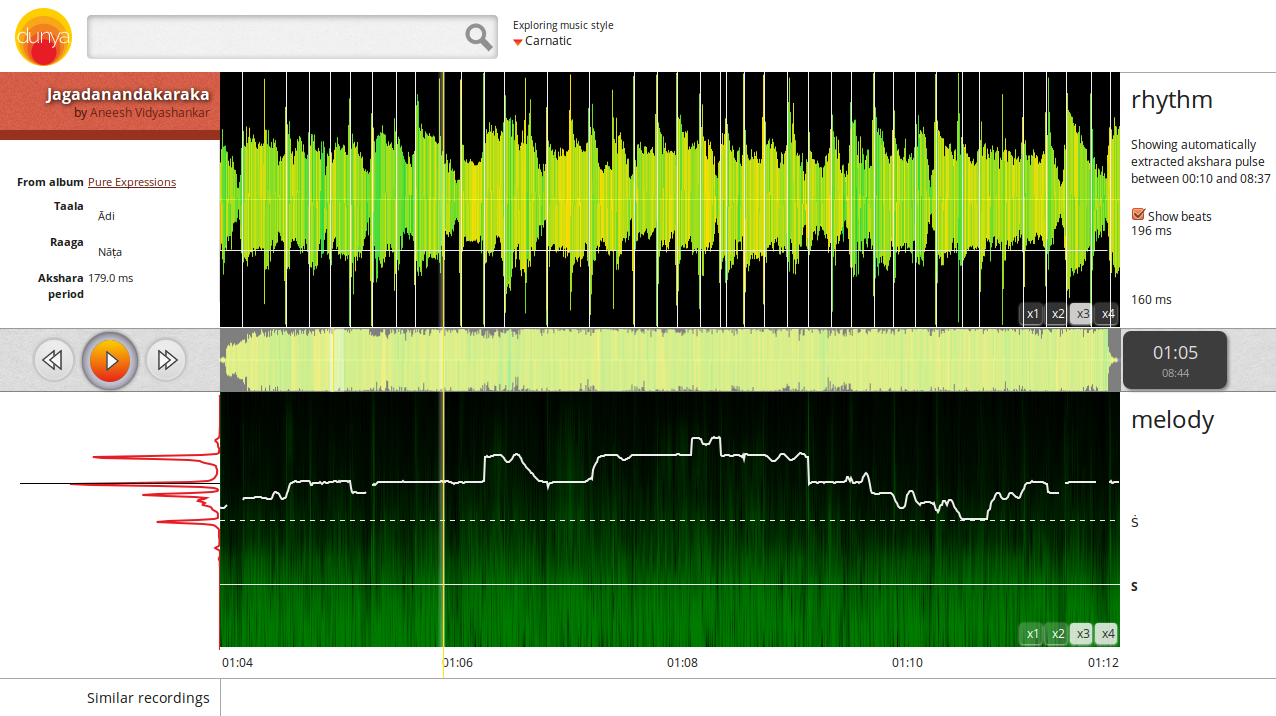
\includegraphics[width=0.90\textheight,angle=90]{screenshots/dunya.png}}%
}%
\caption[A screenshot of the recording page of Dunya]{A screenshot of the recording page of Dunya showing rhythm related metadata in the top panel superimposed on top of the waveform.}\label{fig:dunya:recpage}
\end{figure}
As described earlier, Dunya\footnote{\url{https://dunya.compmusic.upf.edu}} comprises a set of cross-platform open source tools for navigating through music collections in a culture aware and musically relevant way. It is also a test platform to evaluate the research results of CompMusic where users can interact with the music collections under study, helping us to evaluate the research results from a user perspective. Dunya is aimed at the music community of the particular music traditions. It uses the technologies developed for melody and rhythm description to navigate through the audio recordings and through other information items available in a particular music collection. This navigation promotes the discovery of relationships between the different information entities. 

Dunya aggregates music and related metadata from various selected sources such as music archives, Wikipedia and MusicBrainz, and makes it available to users for an enriching and engaging listening experience with music. Audio, automatically and manually extracted features, and curated metadata can also be accessed through Dunya. Dunya has a front end web based tool where users can interactively browse through these music collections. Dunya provides an interface for music similarity based navigation through music collections, and has a detailed recording page that will provide an interactive interface with a visualization of automatically extracted metadata. It will also provide an interface for navigating through the main musically meaningful entities of the specific music culture using characteristic rhythmic and melodic patterns. It also has a back end along with an API that provides access to all these data. Dunya hence acts as the central permanent online repository to store the metadata, audio, annotations and research results. 

The research results from the presented work on rhythm analysis are partly integrated into Dunya, and further integration is in progress. The rhythm analysis tools developed will be a part of the suite of \gls{MIR} tools integrated into Dunya. Essentia\footnote{\url{http://essentia.upf.edu/}} is an audio analysis and audio based \gls{MIR} toolkit~\cite{bogdanov:13:essentiaISMIR,bogdanov:13:essentiaACM}. The Dunya backend uses Essentia to extract features. Hence, specific rhythm extractors from the developed algorithms are also be added to Essentia. 

Drawing information from various data sources and relating them with ontologies, Dunya is the best platform to showcase the tools and algorithms developed as a part of the thesis. A screenshot of the Dunya recording page interface for a Carnatic music recording\footnote{The recording shown in \figref{fig:dunya:recpage} is a violin rendering of the composition Jagadanandakaraka (\url{http://musicbrainz.org/recording/de94ed93-7399-47e3-aa8e-d77b49d94bd3}) from the album Pure expressions (\url{http://musicbrainz.org/release/bcb30e6f-bb13-499d-8e0f-9447af8555a3}) by Aneesh Vidyashankar} is shown in \figref{fig:dunya:recpage}. The recording page shows important rhythm related metadata related to the recording such as \gls{tala} editorial metadata and automatically extracted median \gls{akshara} pulse period ($\iai$). In addition, the waveform panel on the top shows the time varying $\iai$ curve along with \gls{akshara} pulse markers extracted automatically using the approach presented by \citeA{ajay:14:talaTrack}. All of these editorial, automatically extracted, and manually annotated rhythm metadata can also be accessed from the Dunya API. 
% 
\subsection{Sar\={a}ga}
Culture-aware MUsic Technologies (CAMUT) is a project that aims to take the research results of CompMusic to practical real-world commercial applications, aiming to build technologies to foster learning and teaching of Indian music forms. Sar\={a}ga\footnote{Application summary paraphrased from \url{http://musicmuni.com/}} is a music appreciation and infotainment application for students and listeners developed as a part of CAMUT. Sarāga is an android application that provides an enriched listening atmosphere over the open CC collections of Carnatic (\acrshort{CMDo} collection) and Hindustani (\acrshort{HMDo} collection) music. It allows Indian art music connoisseurs and casual listeners to navigate, discover and listen to these music traditions using familiar, relevant and culturally grounded concepts. 

Sarāga includes innovative visualizations in addition to inter and intra-song navigation patterns that present musically rich information to the user. These time synchronized visualizations of musically relevant facets such as melodic patterns, sama locations and sections provide a user with better understanding and appreciation of these music traditions. It additionally features unique compound filters over \glspl{raga}, \glspl{tala}, instruments and artists for finding songs. 
\begin{figure}
\centering
    \subfloat[The entire music piece]{\label{fig:saraga:allsec}
      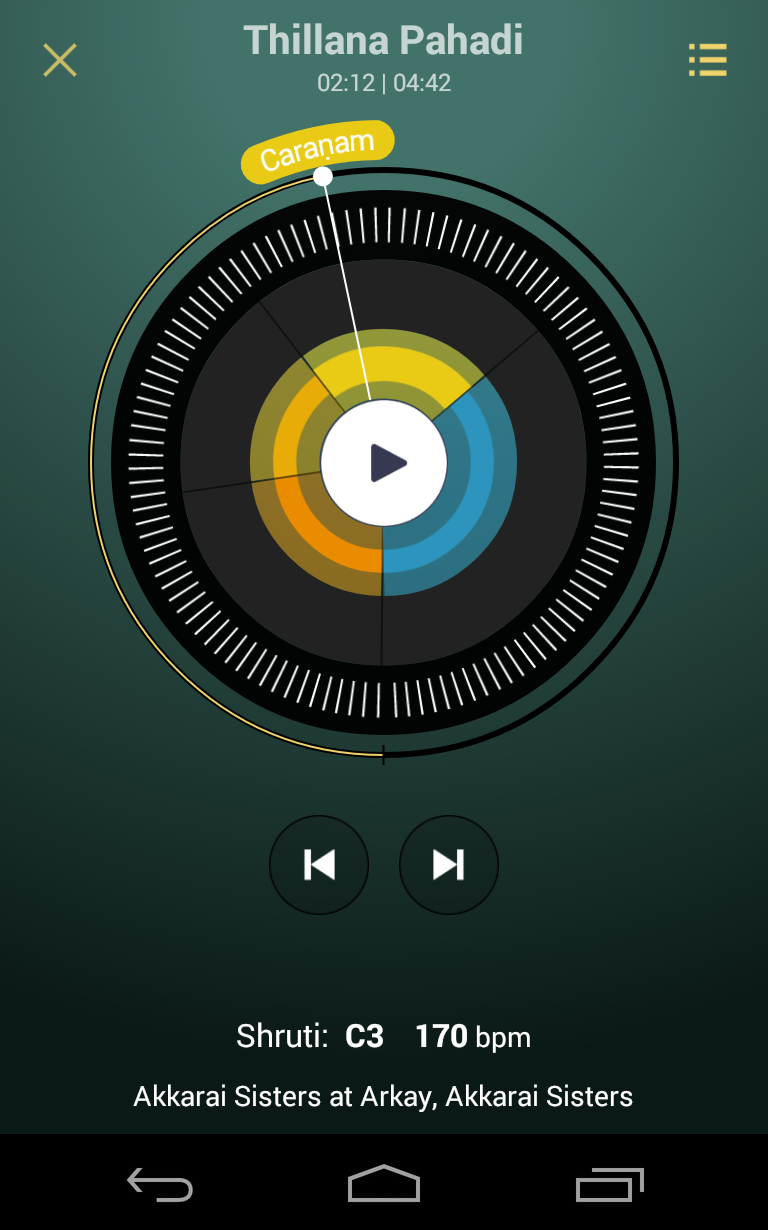
\includegraphics[scale=0.19]{screenshots/saraga-allsec.png}
    } \hspace{0.3cm}
    \subfloat[The \gls{charana} section zoomed]{\label{fig:saraga:charana}
      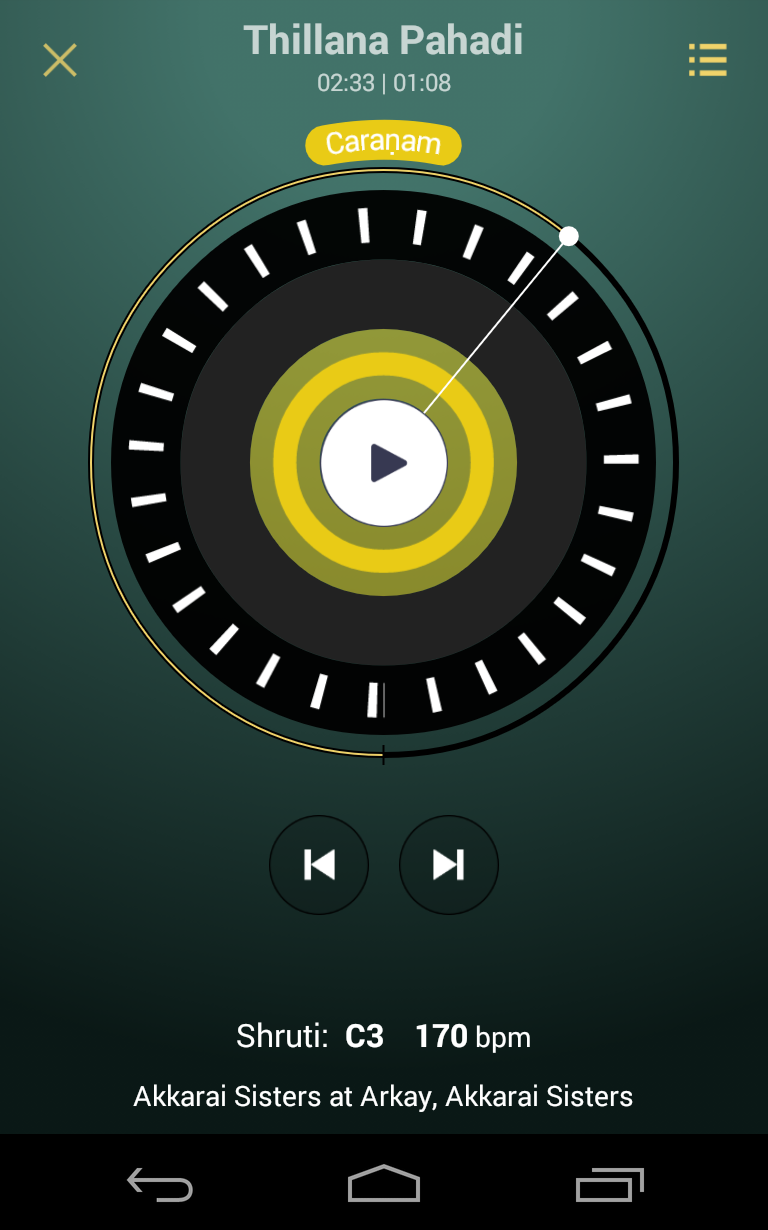
\includegraphics[scale=0.19]{screenshots/saraga-caranam.png}
    } 
\caption[Screenshots of Sar\={a}ga]{Screenshots of the mobile application Sar\={a}ga visualizing a music recording. Panel (a) shows the entire music piece with all the sections, while panel (b) shows the \gls{charana} section zoomed. The sama markers can be seen as white colored ticks on the outer circle. The tempo of the piece is displayed at the bottom of the screen.}\label{fig:saraga:all}
\end{figure}

A screenshot of the application in \figref{fig:saraga:all} shows the rich and novel visualization of a music recording\footnote{The screenshot shows the recording of a \gls{tillana} in \gls{raga} Pahāḍi (\url{http://musicbrainz.org/recording/50c2fea1-d267-4506-a155-73bbefd5da27}) from the album Akkarai Sisters in Arkay (\url{http://musicbrainz.org/release/513e205a-8d71-4d4a-95f7-96d131fa15bc)}} including several different associated metadata. \figref{fig:saraga:allsec} shows all the sections of the piece while \figref{fig:saraga:charana} shows only the \gls{charana} (also called \gls{charana}m) section. The median tempo of the piece is shown as 170 \bpm\ at the bottom of the panel. The whole piece (or a section when zoomed in) is summarized in concentric circles, with white colored time ticks on the outer circle indicating the location of \glspl{sama}. Both the tempo and the \glspl{sama} shown on recordings in Sar\={a}ga have been semi-automatically extracted from audio using \acrshort{pfprior} algorithm with the bar pointer model, and then corrected for any errors manually. 
%\textit{Chapter in brief: Write about applications that have resulted out of the task. And how they can be used for similarity. Discuss applications right now possible. Talk about corpora, dunya, listening tool. Similarity, some basic experiments}

\section{Contributions}
A summary of the specific contributions from the work presented in the dissertation are listed below. %\comment{Give references to sections where they were discussed.}
\subsubsection{Contributions to creating research corpora and datasets}
Building research corpora for \gls{MIR} is one of the primary tasks of CompMusic project. Significant collaborative efforts have been put into building research corpora and datasets, and relevant datasets that have a major contribution by the author are listed below. The links to access all these datasets are provided in \appref{app:resources}. 
\begin{itemize}[leftmargin=*]
	\item CompMusic Carnatic Music Rhythm (\acrshort{CMDf}) dataset: \Gls{tala}, beat and \gls{sama} annotated collection of 176 Carnatic music pieces, built with the support of Vignesh Ishwar, a professional Carnatic musician who also verified the annotations. The dataset has about 16.6 hours of audio with pieces spanning four popular \glspl{tala}. A representative subset of the dataset with 118 pieces (\acrshort{CMDs} dataset) was also built (\secref{sec:cmrdataset}).
	\item CompMusic Hindustani Music Rhythm (\acrshort{HMDf}) dataset: \Gls{taal}, \gls{matra} and \gls{sam} annotated collection of 151 Hindustani music excerpts, built with the support of Kaustuv Kanti Ganguli, a professional Hindustani musician who also verified the annotations. The full dataset has about 5 hours of audio with pieces spanning four popular \glspl{taal} and three different \gls{lay} (tempo classes). Two subsets of the dataset grouped based on \gls{lay}: \acrshort{HMDl} and \acrshort{HMDs} datasets were also built (\secref{sec:hmrdataset}). 
	\item CompMusic Carnatic Creative Commons music (\acrshort{CMDo}) collection: The \gls{sama} annotations for the music pieces of the \acrshort{CMDo} collection in collaboration with Vignesh Ishwar. The collection presently contains over 41 hours of music with 197 pieces and 16880 \gls{sama} annotations (\secref{sec:cmccdataset}).  
	\item CompMusic Hindustani Creative Commons music (\acrshort{HMDo}) collection: The \gls{sam} and section annotations for the music pieces of the \acrshort{HMDo} collection in collaboration with Kaustuv Kanti Ganguli. The collection presently contains over 43 hours of music with over 108 tracks, 11260 \gls{sam} and 215 section annotations (\secref{sec:cmccdataset}). 
	\item CompMusic Mulgaonkar \gls{tabla} solo dataset (\acrshort{TSD}) dataset: A \gls{tabla} solo dataset comprising audio recordings, scores and time aligned syllabic transcriptions of 38 \gls{tabla} solo compositions from different \glspl{gharana} with time-aligned syllabic transcription was built with Swapnil Gupta (\secref{sec:tsdataset}). 
	\item CompMusic \Gls{jingju} percussion pattern (\acrshort{BOPP}) dataset: The \acrshort{BOPP} dataset was built with Rafael Caro Repetto, and consists of 133 audio percussion patterns spanning five different pattern classes, with about 22 minutes of audio and over 2200 percussion syllables (\secref{sec:dataset:bopp}). 
	\item \Gls{jingju} percussion instrument (\acrshort{BOPI}) dataset: Built with Mi Tian at the Centre for Digital Music (C4DM), Queen Mary University of London, the dataset has over 3000 audio examples for four different percussion instrument classes in \gls{jingju} (\secref{sec:dataset:bopi}). 
\end{itemize}
%\acrshort{CMDf} and \acrshort{CMDs} datasets, with help from Vignesh Ishwar. 
%\acrshort{HMDf} and \acrshort{HMDs} and \acrshort{HMDl} datasets, with help from Kaustuv Ganguli
%\acrshort{BOPI} instrument dataset with Mi Tian
%\acrshort{BOPP} pattern dataset with Rafael Caro
%\acrshort{CMDo} sama annotations, along with Vignesh Ishwar
%\acrshort{HMDo} sama annotations, with Kaustuv Ganguli
%Curation of over 100 Hindustani albums in the Dunya collection and adding them to musicbrainz
\subsubsection{Technical and scientific contributions}
\begin{itemize}[leftmargin=*]
	\item Identification of challenges, opportunities and applications of automatic rhythm analysis of Indian art music (\secref{sec:probdef:chopp}). 
	\item Identification of several interesting automatic rhythm analysis problems in Indian art music, along with a review and evaluation of the state of art for some of the tasks, establishing the need for culture-aware methods that can incorporate higher level music information (\chapref{chap:probdef}). 
	\item Engineering formulation of meter analysis (meter inference, meter tracking and informed meter tracking) and percussion pattern discovery (transcription and search) in Indian art music (\secref{sec:probdef:thesis}). 
	\item An illustrative evaluation of the Carnatic and Hindustani music research corpora based on the methodology by \citeA{serra:14:corpus} (\secref{sec:cmcorpora}). 
	\item An illustrative demonstration of the utility of corpora and rhythm analysis tools for a corpus level musicological analysis, as exemplified by rhythmic pattern analysis on Carnatic and Hindustani music rhythm annotated datasets (\secrefs{sec:cmrdataset}{sec:hmrdataset}). 
	\item Bayesian methods for meter analysis in Indian art music: The task of meter analysis addressed for the first time in Carnatic and Hindustani music, developing approaches that are aware of underlying metrical structures and utilize them explicitly. Novel meter analysis model extensions (\momodel\ and \spmodel) and inference extensions are proposed. The novel \spmodel\ shows improvement in tracking long metrical cycles, a task which has been addressed for the first time in \gls{MIR} (\chapref{chap:meterInfTrack}).
	\item Demonstration of the utility of percussion syllables in representation, transcription and discovery of percussion patterns, using a syllabic mapping and grouping system for syllables based on timbral similarity for both \gls{tabla} and mridangam percussion syllables (\chapref{chap:percpatt}, joint work with Swapnil Gupta and IIT Madras CompMusic team). 
	\item Approaches for percussion solo transcription and discovery in syllabic percussion systems, applied on Beijing Opera as a test case and then extended to \gls{tabla} and mridangam percussion solos in Indian art music (\secref{sec:ppclassify:jingju}). 
\end{itemize}
%In summary, we list the specific contributions of the thesis: 
%\begin{enumerate}
%\item A sizeable rhythm annotated audio collection of Hindustani and Carnatic music for research in automatic meter analysis. A consistent and precise machine readable notation for representation of rhythm. 
%\item Engineering formulation of the \gls{MIR} task of meter analysis for Indian art music identifying different challenges. 
%\item Tāla ontologies for both Carnatic and Hindustani Music to provide a semantic framework for inferring relationships between rhythm concepts
%\item Culture-specific signal processing and machine learning algorithms for automatic rhythm annotation of Indian art music.  The important features to extract include the estimation of akṣara/mātrā pulse, beats, sama instants, āvartanaṁ length, naḍe, and eḍupu. 
%\item MIR approaches for rhythm based segmentation of piece to extract rhythm patterns needed to define rhythm similarity
%\item Musically relevant rhythm similarity measures for Indian art music based on empirical ontology based models and thorough listening tests. 
%\item Integration of the developed algorithms into Dunya to improve the functionality of the browser providing an enhanced experience with rhythm annotations, rhythm based segmentation and rhythm similarity. 
%\item Exploring extensions of these approaches and algorithms to other music cultures under the purview of CompMusic such as Makam music of Turkey, Beijing Opera and Andalusian music. 
%\end{enumerate}
\section{Conclusions and summary}
We present a summary, conclusions and the key results from the thesis, organized based on the chapters of the dissertation. Broadly, the dissertation aimed to build culture-aware and domain specific data-driven \gls{MIR} approaches using Bayesian models for automatic rhythm analysis in Indian art music, focusing mainly on the tasks of meter analysis and percussion pattern discovery, with the eventual goal of developing rhythm similarity measures. Such approaches would lead to tools and technologies that can improve our experience with music by helping us to navigate through large music collections in a musically meaningful way, all of it within the sociocultural context of the music culture. The applications lie in enriched music listening, music archival, music learning, musicology, and as pre-processing steps for \gls{MIR} tasks extracting higher level information such as structure and style analysis. 

The dissertation focused on rhythm analysis tasks within the purview of CompMusic project. The scope of the thesis was limited to rhythm analysis in audio collections of Indian art music using Bayesian approaches, emphasizing on data and models. The thesis also addressed the question of the need for culture-aware data-driven approaches to rhythm analysis and its applications. 
% One paragraph per chapter of thesis: What was the motivation, what was done, what are the key conclusions from that chapter. 
%Chap 2: Background to the thesis: State of the art review was done. Background concepts were explained. 

An introduction to rhythm in Indian art music was presented in \chapref{chap:bkgnd} to provide a background to music concepts encountered in the thesis, showing the contrasting differences between several rhythm concepts in Eurogenetic popular music and Indian art music. \Gls{jingju} (Beijing opera) percussion is a suitable case to study percussion patterns and hence a basic introduction to \gls{jingju} was also provided. A review of the state of the art in rhythm analysis tasks in \gls{MIR} provided a basis for understanding relevant rhythm analysis tasks in Indian art music. 

\chapref{chap:probdef} identified some of the unique challenges and opportunities to rhythm analysis in Indian art music. The complexities and characteristics of rhythm in Indian art music make it an ideal candidate for automatic analysis and to push the boundaries of the state of the art in rhythm analysis in \gls{MIR}. Important and relevant rhythm analysis problems within the context of Indian art music were identified and described. An evaluation of the state of the art with some of these problems indicated the need for culture-aware domain specific methods to address these tasks. The set of tasks identified in the chapter will be useful to a researcher looking to solve relevant problems in this new area of research. Definitions relating to rhythm in Indian art music suffered inconsistencies, which were addressed by formulating the research problems of meter analysis and percussion pattern discovery more accurately.

The problem of creating research corpora and datasets for data-driven \gls{MIR}, addressed in \chapref{chap:datasets} shows that significant efforts are needed to build relevant datasets for research. It is possible to build relevant high quality datasets, using a combination of criteria that are used to continuously evaluate the datasets and corpora for their suitability to the tasks at hand. Further, research corpora can be used for corpus level analysis to draw several inferences from it. The dissertation is aimed to be a comprehensive resource for the rhythm related datasets developed as a part of CompMusic, with suggestions on tasks where each of those datasets can be useful. To promote the ideas of open data and reproducible research, all the metadata and some of the audio from the research corpora are openly available through the Dunya API, while the copyrighted commercial audio is easily accessible.

% Chap 5: Meter analysis: Meter analysis used higher level knowledge helps a lot. Several models were discussed. 
Meter analysis was one of the main problems addressed in the thesis. \chapref{chap:meterInfTrack} presented a comprehensive analysis of meter inference, meter tracking, and informed meter tracking in Indian art music. Preliminary experiments showed poor performance with \gls{sama} tracking in Carnatic music, indicating the need for meter analysis methods that can utilize metrical structure information. The bar pointer model is one such Bayesian model that allows for a joint estimation of components of meter and explicitly incorporates the underlying metrical structure. 

An evaluation of the state of the art \bpmodel\ on Indian art music showed the utility of Bayesian models for meter analysis. Novel model extensions (\momodel\ and \spmodel) to improve on \bpmodel\ were proposed. In addition, novel inference extensions based on particle filters for faster inference from these models were also proposed. The algorithms were evaluated for the tasks of meter inference, meter tracking, tempo-informed meter tracking, and tempo-sama-informed meter tracking. The experiments clearly show that incorporating additional \gls{tala} information and making the algorithms more ``informed" improves performance of algorithms. Further, the \spmodel\ shows improvement in tracking long metrical cycles, a task which has been addressed for the first time in \gls{MIR}. 

Contrary to intuition, more number of rhythmic patterns in the observation model did not improve meter analysis performance, which can be attributed to the simplistic spectral flux based audio feature. Further, the \momodel\ and the inference extensions did not show much improvement in performance, but are promising ideas to make inference better and faster with these Bayesian models. The approaches are capable of generalizing to other music cultures, as was demonstrated with the evaluation on the Ballroom dataset. 

A framework for percussion pattern discovery from solo recordings, along with some exploratory experiments for the task was the subject matter of \chapref{chap:percpatt}. Utilizing the syllabic percussion system in Indian art music, we used the onomatopoeic oral-mnemonic syllables to represent, transcribe and search for percussion patterns from audio recordings of percussion solos. A syllabic representation is suitable for timbrally similar percussion patterns and a transcription + search framework was explored for discovery of patterns. 

Preliminary experiments on percussion pattern transcription and classification were presented on \gls{jingju} percussion patterns. The approach was then extended to pattern discovery by transcription followed by approximate search on \gls{tabla} and mridangam solo recordings. The transcription was based on a speech recognition framework using timbral syllable models along with a simple language model. A set of query patterns were automatically derived from symbolic syllabic scores. To make the approach robust to errors in automatic transcription, an approximate search algorithm (\gls{RLCS}) was used to search for these query patterns in transcribed recordings. 

Preliminary experiments on the \acrshort{TSD} and \acrshort{UMSD} datasets showed the large number of insertion errors and the need for approximate search algorithms. Exact string search algorithm had a good precision but a poor recall due to all the transcription errors. An approximate string search algorithm \gls{RLCS} showed improvement in pattern recall with the \acrshort{TSD} dataset that included full length compositions. The \acrshort{UMSD} dataset consists of short audio files segmented by phrases and hence \gls{RLCS} did not show much improvement in overall f-measure over an exact string search. 

The variants of \gls{RLCS} need to be further explored and improved. For the task, the combination of transcription + search for the problem is a promising approach, while further experiments with a comprehensive evaluation is needed to make stronger claims on performance and suggest improvements. 
%
\section{Future directions}
There are several directions for future work based on the thesis. One of the goals of the dissertation was to present relevant research problems in rhythm analysis of Indian art music. Some of these problems presented in \chapref{chap:probdef} are a good start to extend the work presented in the dissertation. Several rhythm tasks for Indian art music were proposed in \chapref{chap:probdef}, while only a few of them were addressed in the thesis. The problems such as building rhythm ontologies and rhythm based segmentation have received little attention from the research community so far. Both are relevant areas of research with a potential to be explored in the future. 

The goal of automatic rhythm analysis is to define musically relevant rhythm similarity measures, a topic that has not been addressed in the dissertation. Using both rhythmic structures and patterns extracted from audio to define better measures is an important part of future work. In addition, the work in the thesis used only audio recordings to extract meaningful rhythm information. However, using additional metadata (such as lyrics, scores, editorial metadata) along with audio features and combining them with suitable rhythm ontologies can lead to better similarity measures, which is to be explored as a part of future work. 

The sizeable curated research corpora and datasets built in CompMusic provide an immense opportunity to be utilized for a variety of research problems in the future. The availability of the datasets now opens up the possibility of significant data-driven automatic rhythm analysis research in these music cultures. The problems that can use these datasets were detailed in \chapref{chap:datasets}. In addition, the Creative Commons music collections developed for Carnatic and Hindustani music can be used to build open data and algorithms without restrictive copyright issues. 

The research corpora evolves over time. Improving the research corpora sustainably and building additional datasets for automatic rhythm analysis are important tasks for future. The use of these datasets for musicological research was hinted in our experiments, but a rigorous study of suitability of the corpora and datasets for musicology, and its adoption for musicological studies is one direction to pursue. 

Meter analysis tasks such as meter inference and tracking were addressed in detail in the dissertation. However, there are several open questions that still have to be more rigorously answered. The experiments need to be extended to full length music pieces from the present experiments on shorter excerpts, to make it more practical. A part of immediate future work would be to evaluate it further on larger Indian music datasets. The \spmodel\ for meter analysis showed significant promise in tracking a wide range of metrical structures in both Carnatic and Hindustani music. Formal evaluations on its extendability to other music cultures is an important part of future work. The model and inference extensions need to be analyzed further to improve their performance. The use of spectral flux feature for meter analysis is limiting. Developing better audio features that can perhaps also include information from other dimensions such as melody and lyrics are to be further explored. 

Percussion pattern discovery was a problem that was addressed to a lesser extent in the dissertation with only preliminary results presented on small datasets. While the framework using syllabic representation for percussion patterns is promising, an extensive evaluation on larger datasets spanning different instrument timbres, playing styles, schools (\glspl{gharana}), and variability in patterns is to be done in the future. Better transcription can be achieved in real world scenarios with the availability of such diverse data to build acoustic and language models. Approximate string search using \gls{RLCS} shows promise in searching for short query patterns in longer transcribed audio recordings, while some improvements suggested to it need further exploration to make the search algorithm robust to transcription errors. 

The tasks of meter analysis and percussion transcription and discovery were addressed as independent tasks in the thesis, while there is also significant interplay between the tasks. Meter analysis could benefit from percussion instrument timbre based features to track metrical structures (the strokes of \gls{tabla} played in a \gls{theka} are indicative of position in the \gls{taal} cycle). Percussion pattern discovery can benefit significantly if the \gls{sama} and beat information is available, since percussion patterns are often aligned with beats (and sometimes \gls{sama}) of the \gls{tala}. New approaches that can address the two tasks together and build joint analysis algorithms are promising. 

Integration of these algorithms and methods into practical applications requires additional effort to understand the gaps between research tasks and practical needs. Tools such as Dunya aim to bridge that gap by providing an evaluation framework for research algorithms. In the future, an integration of all the described rhythm analysis approaches into Dunya is necessary and it helps to improve the algorithms through user feedback, while aiming to provide users with an engaging experience with large collections of music. 

We sincerely believe that the dissertation has opened up the new area of research in automatic rhythm analysis of Indian art music. With several challenging and interesting research problems in the area, there is significant scope and potential for novel approaches and methodologies to solve these problems. The future directions discussed here provide pointers for further research in the field, and this is perhaps where a new PhD thesis can begin! 